\documentclass[man, fleqn, noextraspace]{apa6}
\usepackage{lmodern}
\usepackage{amssymb,amsmath}
\usepackage{ifxetex,ifluatex}
\usepackage{fixltx2e} % provides \textsubscript
\ifnum 0\ifxetex 1\fi\ifluatex 1\fi=0 % if pdftex
  \usepackage[T1]{fontenc}
  \usepackage[utf8]{inputenc}
\else % if luatex or xelatex
  \ifxetex
    \usepackage{mathspec}
  \else
    \usepackage{fontspec}
  \fi
  \defaultfontfeatures{Ligatures=TeX,Scale=MatchLowercase}
\fi
% use upquote if available, for straight quotes in verbatim environments
\IfFileExists{upquote.sty}{\usepackage{upquote}}{}
% use microtype if available
\IfFileExists{microtype.sty}{%
\usepackage{microtype}
\UseMicrotypeSet[protrusion]{basicmath} % disable protrusion for tt fonts
}{}
\usepackage{hyperref}
\hypersetup{unicode=true,
            pdftitle={Data Visdualization on Madarin Vowels},
            pdfauthor={Teresa Chen, Jun Lun, Steffi Hung, \& Ting-fen Lin},
            pdfkeywords={Madarin, Vowels, Native speaker, Non-native speaker},
            pdfborder={0 0 0},
            breaklinks=true}
\urlstyle{same}  % don't use monospace font for urls
\usepackage{graphicx,grffile}
\makeatletter
\def\maxwidth{\ifdim\Gin@nat@width>\linewidth\linewidth\else\Gin@nat@width\fi}
\def\maxheight{\ifdim\Gin@nat@height>\textheight\textheight\else\Gin@nat@height\fi}
\makeatother
% Scale images if necessary, so that they will not overflow the page
% margins by default, and it is still possible to overwrite the defaults
% using explicit options in \includegraphics[width, height, ...]{}
\setkeys{Gin}{width=\maxwidth,height=\maxheight,keepaspectratio}
\IfFileExists{parskip.sty}{%
\usepackage{parskip}
}{% else
\setlength{\parindent}{0pt}
\setlength{\parskip}{6pt plus 2pt minus 1pt}
}
\setlength{\emergencystretch}{3em}  % prevent overfull lines
\providecommand{\tightlist}{%
  \setlength{\itemsep}{0pt}\setlength{\parskip}{0pt}}
\setcounter{secnumdepth}{0}
% Redefines (sub)paragraphs to behave more like sections
\ifx\paragraph\undefined\else
\let\oldparagraph\paragraph
\renewcommand{\paragraph}[1]{\oldparagraph{#1}\mbox{}}
\fi
\ifx\subparagraph\undefined\else
\let\oldsubparagraph\subparagraph
\renewcommand{\subparagraph}[1]{\oldsubparagraph{#1}\mbox{}}
\fi

%%% Use protect on footnotes to avoid problems with footnotes in titles
\let\rmarkdownfootnote\footnote%
\def\footnote{\protect\rmarkdownfootnote}


  \title{Data Visdualization on Madarin Vowels}
    \author{Teresa Chen\textsuperscript{3}, Jun Lun\textsuperscript{2}, Steffi
Hung\textsuperscript{2}, \& Ting-fen Lin\textsuperscript{1}}
    \date{}
  
\shorttitle{Final Project in EDLD 610: Introduction to Data Science with R}
\affiliation{
\vspace{0.5cm}
\textsuperscript{1} Department of Human Physiology\\\textsuperscript{2} Department of East Asia Linguistic Language\\\textsuperscript{3} Department of Communication Disorder}
\keywords{Madarin, Vowels, Native speaker, Non-native speaker}
\usepackage{csquotes}
\usepackage{upgreek}
\captionsetup{font=singlespacing,justification=justified}

\usepackage{longtable}
\usepackage{lscape}
\usepackage{multirow}
\usepackage{tabularx}
\usepackage[flushleft]{threeparttable}
\usepackage{threeparttablex}

\newenvironment{lltable}{\begin{landscape}\begin{center}\begin{ThreePartTable}}{\end{ThreePartTable}\end{center}\end{landscape}}

\makeatletter
\newcommand\LastLTentrywidth{1em}
\newlength\longtablewidth
\setlength{\longtablewidth}{1in}
\newcommand{\getlongtablewidth}{\begingroup \ifcsname LT@\roman{LT@tables}\endcsname \global\longtablewidth=0pt \renewcommand{\LT@entry}[2]{\global\advance\longtablewidth by ##2\relax\gdef\LastLTentrywidth{##2}}\@nameuse{LT@\roman{LT@tables}} \fi \endgroup}


\DeclareDelayedFloatFlavor{ThreePartTable}{table}
\DeclareDelayedFloatFlavor{lltable}{table}
\DeclareDelayedFloatFlavor*{longtable}{table}
\makeatletter
\renewcommand{\efloat@iwrite}[1]{\immediate\expandafter\protected@write\csname efloat@post#1\endcsname{}}
\makeatother
\usepackage{lineno}

\linenumbers

\authornote{Steffi and Jun are the owner of the dataset. They
have the correct permissions to make the dataset public.

Correspondence concerning this article should be addressed to Teresa
Chen, Rm.52 Gerlnger Annex, University of Oregon, OR 9740. E-mail:
\href{mailto:szuhuac@uoregon.edu}{\nolinkurl{szuhuac@uoregon.edu}}}

\abstract{
One or two sentences providing a \textbf{basic introduction} to the
field, comprehensible to a scientist in any discipline.

Two to three sentences of \textbf{more detailed background},
comprehensible to scientists in related disciplines.

One sentence clearly stating the \textbf{general problem} being
addressed by this particular study.

One sentence summarizing the main result (with the words ``\textbf{here
we show}'' or their equivalent).

Two or three sentences explaining what the \textbf{main result} reveals
in direct comparison to what was thought to be the case previously, or
how the main result adds to previous knowledge.

One or two sentences to put the results into a more \textbf{general
context}.

Two or three sentences to provide a \textbf{broader perspective},
readily comprehensible to a scientist in any discipline.


}

\begin{document}
\maketitle

{
\setcounter{tocdepth}{5}
\tableofcontents
}
\newpage

\section{Methods}\label{methods}

We report how we determined our sample size, all data exclusions (if
any), all manipulations, and all measures in the study.

\subsection{Participants}\label{participants}

\subsection{Material}\label{material}

\subsection{Procedure}\label{procedure}

\subsection{Data analysis}\label{data-analysis}

We used R (Version 3.4.2; R Core Team, 2017) and the R-packages
\emph{bindrcpp} (Version 0.2.2; Müller, 2018), \emph{dplyr} (Version
0.7.6; Wickham, François, Henry, \& Müller, 2018), \emph{forcats}
(Version 0.3.0; Wickham, 2018a), \emph{ggplot2} (Version 3.0.0; Wickham,
2016), \emph{here} (Version 0.1; Müller, 2017), \emph{janitor} (Version
1.1.1; Firke, 2018), \emph{kableExtra} (Version 0.9.0; Zhu, 2018),
\emph{knitr} (Version 1.20; Xie, 2015), \emph{papaja} (Version
0.1.0.9842; Aust \& Barth, 2018), \emph{purrr} (Version 0.2.5; Henry \&
Wickham, 2018), \emph{readr} (Version 1.1.1; Wickham, Hester, \&
Francois, 2017), \emph{rio} (Version 0.5.10; C.-h. Chan, Chan, Leeper,
\& Becker, 2018), \emph{stringr} (Version 1.3.1; Wickham, 2018b),
\emph{tibble} (Version 1.4.2; Müller \& Wickham, 2018), \emph{tidyr}
(Version 0.8.1; Wickham \& Henry, 2018), \emph{tidyverse} (Version
1.2.1; Wickham, 2017), and \emph{tinytex} (Version 0.8; Xie, 2018) for
all our analyses.

\section{Results}\label{results}

\begin{figure}
\centering
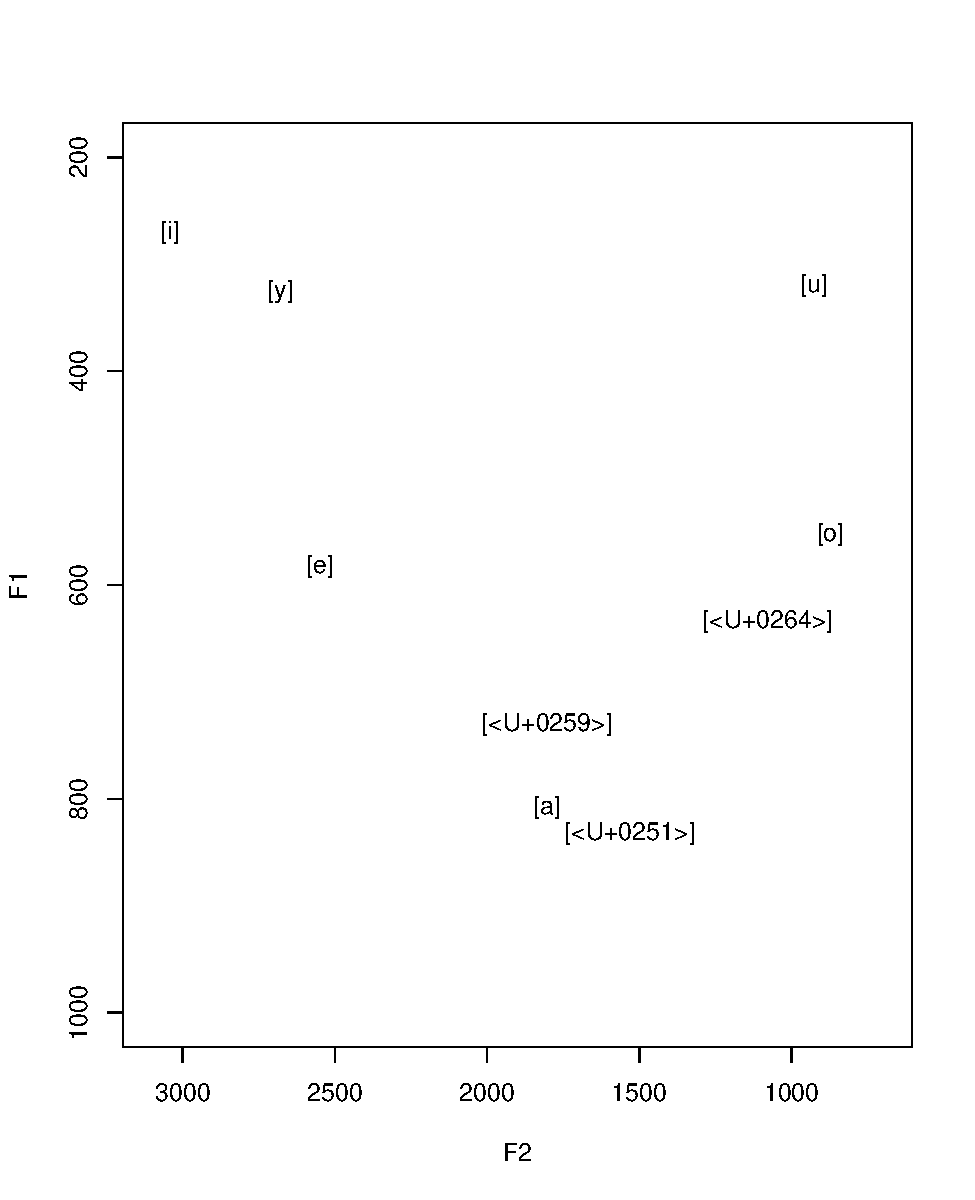
\includegraphics{Vowel_v2_files/figure-latex/figure1-1.pdf}
\caption{}
\end{figure}

\begin{table}

\caption{\label{tab:table1}Formant by volwels among non-native and native groups}
\centering
\begin{tabular}[t]{llrrrr}
\toprule
group & vowel & F1\_mean & F2\_mean & F1\_sd & F2\_sd\\
\midrule
NNS & ai & 913.33 & 1513.83 & 47.14 & 161.28\\
NNS & ao & 901.50 & 1377.00 & 63.86 & 107.69\\
NNS & e & 640.33 & 1702.33 & 70.43 & 238.62\\
NNS & en & 651.33 & 1980.00 & 88.59 & 166.70\\
NNS & wo & 551.50 & 1043.67 & 49.79 & 61.90\\
\addlinespace
NNS & wu & 416.00 & 1122.83 & 69.62 & 196.96\\
NNS & ye & 520.67 & 2320.00 & 65.50 & 95.07\\
NNS & yi & 335.67 & 2646.50 & 46.03 & 100.61\\
NNS & yu & 321.50 & 1806.83 & 31.25 & 186.00\\
NS & ai & 910.33 & 1655.50 & 115.38 & 142.20\\
\addlinespace
NS & ao & 848.00 & 1305.17 & 59.50 & 147.96\\
NS & e & 596.83 & 1289.67 & 105.92 & 152.62\\
NS & en & 717.67 & 1850.50 & 40.10 & 101.96\\
NS & wo & 554.50 & 908.67 & 48.53 & 76.63\\
NS & wu & 335.00 & 840.00 & 15.63 & 56.02\\
\addlinespace
NS & ye & 556.83 & 2486.50 & 38.02 & 128.39\\
NS & yi & 308.33 & 2916.17 & 30.23 & 73.78\\
NS & yu & 309.17 & 2420.83 & 15.17 & 237.25\\
\bottomrule
\end{tabular}
\end{table}

\begin{figure}
\centering
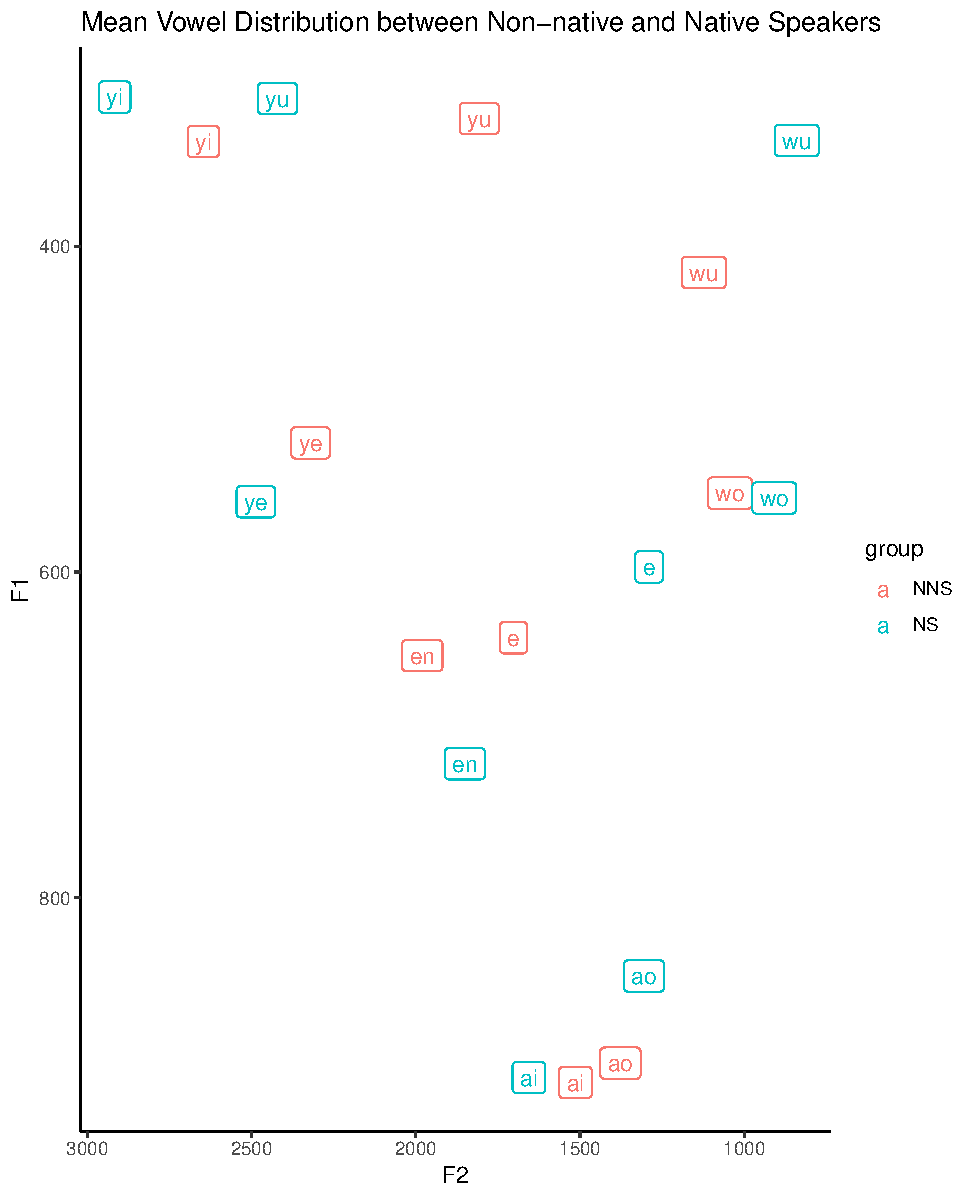
\includegraphics{Vowel_v2_files/figure-latex/figure2-1.pdf}
\caption{}
\end{figure}

\begin{figure}
\centering
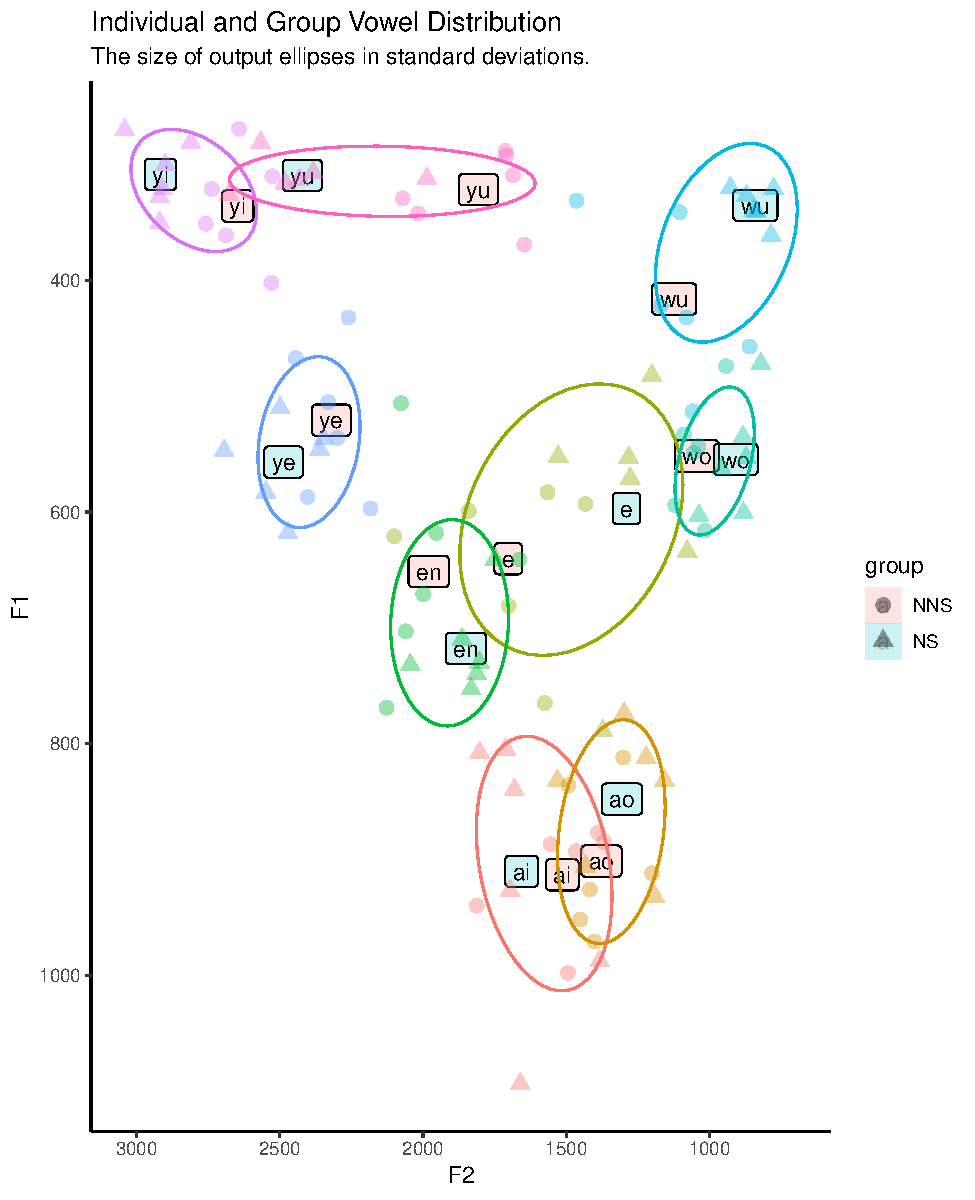
\includegraphics{Vowel_v2_files/figure-latex/figure3-1.pdf}
\caption{}
\end{figure}

\section{Discussion}\label{discussion}

\newpage

\section{References}\label{references}

\begingroup
\setlength{\parindent}{-0.5in} \setlength{\leftskip}{0.5in}

\hypertarget{refs}{}
\hypertarget{ref-R-papaja}{}
Aust, F., \& Barth, M. (2018). \emph{papaja: Create APA manuscripts with
R Markdown}. Retrieved from \url{https://github.com/crsh/papaja}

\hypertarget{ref-R-rio}{}
Chan, C.-h., Chan, G. C., Leeper, T. J., \& Becker, J. (2018).
\emph{Rio: A swiss-army knife for data file i/o}.

\hypertarget{ref-R-janitor}{}
Firke, S. (2018). \emph{Janitor: Simple tools for examining and cleaning
dirty data}. Retrieved from
\url{https://CRAN.R-project.org/package=janitor}

\hypertarget{ref-R-purrr}{}
Henry, L., \& Wickham, H. (2018). \emph{Purrr: Functional programming
tools}. Retrieved from \url{https://CRAN.R-project.org/package=purrr}

\hypertarget{ref-R-here}{}
Müller, K. (2017). \emph{Here: A simpler way to find your files}.
Retrieved from \url{https://CRAN.R-project.org/package=here}

\hypertarget{ref-R-bindrcpp}{}
Müller, K. (2018). \emph{Bindrcpp: An 'rcpp' interface to active
bindings}. Retrieved from
\url{https://CRAN.R-project.org/package=bindrcpp}

\hypertarget{ref-R-tibble}{}
Müller, K., \& Wickham, H. (2018). \emph{Tibble: Simple data frames}.
Retrieved from \url{https://CRAN.R-project.org/package=tibble}

\hypertarget{ref-R-base}{}
R Core Team. (2017). \emph{R: A language and environment for statistical
computing}. Vienna, Austria: R Foundation for Statistical Computing.
Retrieved from \url{https://www.R-project.org/}

\hypertarget{ref-R-ggplot2}{}
Wickham, H. (2016). \emph{Ggplot2: Elegant graphics for data analysis}.
Springer-Verlag New York. Retrieved from \url{http://ggplot2.org}

\hypertarget{ref-R-tidyverse}{}
Wickham, H. (2017). \emph{Tidyverse: Easily install and load the
'tidyverse'}. Retrieved from
\url{https://CRAN.R-project.org/package=tidyverse}

\hypertarget{ref-R-forcats}{}
Wickham, H. (2018a). \emph{Forcats: Tools for working with categorical
variables (factors)}. Retrieved from
\url{https://CRAN.R-project.org/package=forcats}

\hypertarget{ref-R-stringr}{}
Wickham, H. (2018b). \emph{Stringr: Simple, consistent wrappers for
common string operations}. Retrieved from
\url{https://CRAN.R-project.org/package=stringr}

\hypertarget{ref-R-tidyr}{}
Wickham, H., \& Henry, L. (2018). \emph{Tidyr: Easily tidy data with
'spread()' and 'gather()' functions}. Retrieved from
\url{https://CRAN.R-project.org/package=tidyr}

\hypertarget{ref-R-dplyr}{}
Wickham, H., François, R., Henry, L., \& Müller, K. (2018). \emph{Dplyr:
A grammar of data manipulation}. Retrieved from
\url{https://CRAN.R-project.org/package=dplyr}

\hypertarget{ref-R-readr}{}
Wickham, H., Hester, J., \& Francois, R. (2017). \emph{Readr: Read
rectangular text data}. Retrieved from
\url{https://CRAN.R-project.org/package=readr}

\hypertarget{ref-R-knitr}{}
Xie, Y. (2015). \emph{Dynamic documents with R and knitr} (2nd ed.).
Boca Raton, Florida: Chapman; Hall/CRC. Retrieved from
\url{https://yihui.name/knitr/}

\hypertarget{ref-R-tinytex}{}
Xie, Y. (2018). \emph{Tinytex: Helper functions to install and maintain
'tex live', and compile 'latex' documents}. Retrieved from
\url{https://CRAN.R-project.org/package=tinytex}

\hypertarget{ref-R-kableExtra}{}
Zhu, H. (2018). \emph{KableExtra: Construct complex table with 'kable'
and pipe syntax}. Retrieved from
\url{https://CRAN.R-project.org/package=kableExtra}

\endgroup


\end{document}
